\documentclass[a4paper,12pt]{article}

\usepackage{cmap}		
\usepackage[utf8]{inputenc}			
\usepackage[english,russian]{babel}
\usepackage{framed}
\usepackage{hyperref}
\usepackage{amsmath}
\usepackage{graphicx}
\usepackage[colorinlistoftodos]{todonotes}
\usepackage{wrapfig}
\usepackage{lipsum}
\usepackage{color}
\usepackage{indentfirst}
\usepackage{times}
\usepackage{textcomp}
\usepackage{float}
\usepackage{listings}
\usepackage{xcolor}
\usepackage[T1]{fontenc}

\usepackage{morewrites}

\usepackage[pdf]{graphviz}
\usepackage{xpatch}
\makeatletter
\newcommand*{\addFileDependency}[1]{% argument=file name and extension
  \typeout{(#1)}
  \@addtofilelist{#1}
  \IfFileExists{#1}{}{\typeout{No file #1.}}
}
\makeatother
\xpretocmd{\digraph}{\addFileDependency{#2.dot}}{}{}

\usepackage[autosize]{dot2texi}
\usepackage{tikz}
\usetikzlibrary{shapes,arrows}

\newcommand{\HRule}{\rule{\linewidth}{0.5mm}}

\begin{document}

\begin{titlepage}
\begin{center}



% Upper part of the page. The '~' is needed because \\
% only works if a paragraph has started.
\textsc{\Large НАЦИОНАЛЬНЫЙ ИССЛЕДОВАТЕЛЬСКИЙ УНИВЕРСИТЕТ}\\
\textsc{\Large "МЭИ"}\\[1cm]


\includegraphics[width=0.8\textwidth]{img/logo.png}~\\[1cm]

\textsc{\Large Теоретические модели вычисления}\\[0.5cm]

% Title
\HRule \\[0.4cm]
{ \LARGE \bfseries ДЗ №1: Регулярные языки и конечные автоматы \\[0.4cm] }

\HRule \\[1.5cm]

% Author and supervisor
\noindent
\begin{minipage}{0.4\textwidth}
\begin{flushleft} \large
\emph{Студент:}\\
Николаев \textsc{Ю.~С.}
\end{flushleft}
\end{minipage}%
\begin{minipage}{0.4\textwidth}
\begin{flushright} \large
\emph{GitHub:} \\
\href{https://github.com/NRU-MPEI-IMAI/regular-languages-and-finite-machines-nikolaevje}{@nikolaevje}
\end{flushright}
\end{minipage}

\vfill

% Bottom of the page
{\large Москва, 2022}

\end{center}
\end{titlepage}

\newpage
\tableofcontents

\newpage

\section{Построить конечный автомат, распознающий язык}

\subsection{$L = \{\omega \in \{a, b, c\}^* \: | \: |\omega|_c = 1\}$}
\begin{center}
    \digraph{g11}{
        size="6,6";
        rankdir="LR";
        0 [shape=point];
        1 [shape=circle];
        2 [shape=doublecircle];
        0 -> 1;
        1 -> 1 [label="a, b"];
        1 -> 2 [label="c"];
        2 -> 2 [label="a, b"];
    }
\end{center}

\subsection{$L = \{\omega \in \{a, b\}^{*} \: | \: |\omega|_a \leq 2, |\omega|_b \geq 2, \}$}

\begin{center}
    $|\omega|_a \leq 2 \Rightarrow A_1 = \{\Sigma = \{a, b\}, Q_1 = \{1, 2, 3\}, 1, T_1 = \{1, 2, 3\}, \delta_1 \}$
    
    \digraph[scale=0.8]{g120}{
        size="6,6";
        rankdir="LR";
        node [shape=point]; 0;
        node [shape=doublecircle] 1 2 3;
        0 -> 1;
        1 -> 1 [label="b"];
        1 -> 2 [label="a"];
        2 -> 2 [label="b"];
        2 -> 3 [label="a"];
        3 -> 3 [label="b"];
    }
    
    $|\omega|_b \geq 2 \Rightarrow A_2 = \{\Sigma = \{a, b\}, Q_2 = \{1, 2, 3\}, 1, T_2 = \{3\}, \delta_2 \}$
    \digraph[scale=0.8]{g121}{
        size="6,6";
        rankdir="LR";
        node [shape=point]; 0;
        node [shape=circle]; 1 2;
        node [shape=doublecircle]; 3;
        0 -> 1;
        1 -> 1 [label="a"];
        1 -> 2 [label="b"];
        2 -> 2 [label="a"];
        2 -> 3 [label="b"];
        3 -> 3 [label="a, b"];
    }
\end{center}
    \newpage
    
    Построим прямое произведение:
    \begin{enumerate}
        \item $\Sigma = \{a, b\}$
        \item $Q = \{(1, 1), (1, 2), (1, 3), (2, 1), (2, 2), (2, 3), (3, 1), (3, 2), (3, 3)\}$
        \item $S = \{(1, 1)\}$
        \item $T = \{(1, 3), (2, 3), (3, 3)\}$
        \item $\delta:$
        \begin{tabular}{|c|c|c|c|}
            \hline
            A_1 & A_2 & a & b  \\ \hline
            1 & 1 & 21 & 12  \\ \hline
            1 & 2 & 22 & 13  \\ \hline
            1 & 3 & 23 & 13  \\ \hline
            2 & 1 & 31 & 22  \\ \hline
            2 & 2 & 32 & 23  \\ \hline
            2 & 3 & 33 & 23  \\ \hline
            3 & 1 & - & 32  \\ \hline
            3 & 2 & - & 33  \\ \hline
            3 & 3 & - & 33  \\
            \hline
        \end{tabular}
    \end{enumerate}
    
\begin{center}
    \digraph[scale=0.8]{g12}{
        size="6,6";
        rankdir="LR";
        node [shape=point]; 0;
        node [shape=circle]; 11 12 21 22 31 32;
        node [shape=doublecircle]; 13 23 33;
        0 -> 11;
        11 -> 21 [label="a"];
        11 -> 12 [label="b"];
        12 -> 22 [label="a"];
        12 -> 13 [label="b"];
        13 -> 23 [label="a"];
        13 -> 13 [label="b"];
        21 -> 31 [label="a"];
        21 -> 22 [label="b"];
        22 -> 32 [label="a"];
        22 -> 23 [label="b"];
        23 -> 33 [label="a"];
        23 -> 23 [label="b"];
        31 -> 32 [label="b"];
        32 -> 33 [label="b"];
        33 -> 33 [label="b"];
    }
\end{center}

\newpage

\subsection{$L = \{\omega \in \{a, b\}^{*} \: | \: |\omega|_a \neq |\omega|_b\}$}

Как мы помним из лекции, конечные автоматы - беспамятные у****ки. 

Собственно, этот пример требует запоминать количество символов.

Невозможно построить автомат.

\subsection{$L = \{\omega \in \{a, b\}^{*} \: | \: \omega\omega = \omega\omega\omega\}$}

Существует единственное такое слово - пустое.

\begin{center}
    \digraph{g14}{
        size="6,6";
        rankdir="LR";
        0 [shape=point];
        1 [shape=doublecircle];
        0 -> 1;
    }
\end{center}

\newpage

\section{Построить конечный автомат, используя прямое произведение}

\subsection{$L_1 = \{\omega \in \{a, b\}^{*} \: | \: |\omega|_a \geq 2 \land |\omega|_b \geq 2\}$}

Есть два автомата:

\begin{center}
    $|\omega|_a \geq 2 \Rightarrow A_1 = \{\Sigma = \{a, b\}, Q_1 = \{1, 2, 3\}, 1, T_1 = \{3\}, \delta_1 \}$
    
    \digraph[scale=0.8]{g210}{
        size="6,6";
        rankdir="LR";
        node [shape=point]; 0;
        node [shape=circle]; 1 2;
        node [shape=doublecircle]; 3;
        0 -> 1;
        1 -> 1 [label="b"];
        1 -> 2 [label="a"];
        2 -> 2 [label="b"];
        2 -> 3 [label="a"];
        3 -> 3 [label="a, b"];
    }
    
    $|\omega|_b \geq 2 \Rightarrow A_2 = \{\Sigma = \{a, b\}, Q_2 = \{1, 2, 3\}, 1, T_2 = \{3\}, \delta_2 \}$
    
    \digraph[scale=0.8]{g211}{
        size="6,6";
        rankdir="LR";
        node [shape=point]; 0;
        node [shape=circle]; 1 2;
        node [shape=doublecircle]; 3;
        0 -> 1;
        1 -> 1 [label="a"];
        1 -> 2 [label="b"];
        2 -> 2 [label="a"];
        2 -> 3 [label="b"];
        3 -> 3 [label="a, b"];
    }
\end{center}

\newpage

    Прямое произведение:
    
    \begin{enumerate}
        \item $\Sigma = \{a, b\}$
        \item $Q = \{(1, 1), (1, 2), (1, 3), (2, 1), (2, 2), (2, 3), (3, 1), (3, 2), (3, 3)\}$
        \item $S = \{(1, 1)\}$
        \item $T = \{(3, 3)\}$
        \item $\delta:$
        \begin{tabular}{|c|c|c|c|}
            \hline
            $A_1$ & $A_2$ & a & b  \\ \hline
            1 & 1 & 21 & 12  \\ \hline
            1 & 2 & 22 & 13  \\ \hline
            1 & 3 & 23 & 13  \\ \hline
            2 & 1 & 31 & 22  \\ \hline
            2 & 2 & 32 & 23  \\ \hline
            2 & 3 & 33 & 23  \\ \hline
            3 & 1 & 31 & 32  \\ \hline
            3 & 2 & 32 & 33  \\ \hline
            3 & 3 & 33 & 33  \\
            \hline
    \end{tabular}
    \end{enumerate}
    
    \begin{center}
        \digraph[scale=0.8]{g21}{
            size="6,6";
            rankdir="LR";
            node [shape=point]; 0;
            node [shape=circle]; 11 12 13 21 22 23 31 32;
            node [shape=doublecircle]; 33;
            0 -> 11;
            11 -> 21 [label="a"];
            11 -> 12 [label="b"];
            12 -> 22 [label="a"];
            12 -> 13 [label="b"];
            13 -> 23 [label="a"];
            13 -> 13 [label="b"];
            21 -> 31 [label="a"];
            21 -> 22 [label="b"];
            22 -> 32 [label="a"];
            22 -> 23 [label="b"];
            23 -> 33 [label="a"];
            23 -> 23 [label="b"];
            31 -> 31 [label="a"];
            31 -> 32 [label="b"];
            32 -> 33 [label="a, b"];
            33 -> 33 [label="a, b"];
        }
    \end{center}

\newpage

\subsection{$L_2 = \{\omega \in \{a, b\}^{*} \: | \: |\omega| \geq 3 \land |\omega| \: \text{нечетное}\}$}

    $|\omega| \geq 3 \Rightarrow A_1 = \{\Sigma = \{a, b\}, Q_1 = \{1, 2, 3, 4\}, S_1 =\{ 1\}, T_1 = \{4\}, \delta_1 \}$ 
    
    \begin{center}
        \digraph{g220}{
            size="6,6";
            rankdir="LR";
            node [shape=point]; 0;
            node [shape=circle]; 1 2,3;
            node [shape=doublecircle]; 4;
            0 -> 1;
            1 -> 2 [label="a,b"];
            2 -> 3 [label="a,b"];
            3 -> 4 [label="a,b"];
            4 -> 4 [label="a,b"];
        }
    \end{center}
    
    $|\omega| \: \text{нечетное} \Rightarrow A_2 = \{\Sigma = \{a, b\}, Q_2 = \{1, 2\}, S_2 =\{ 1\}, T_2 = \{2\}, \delta_2\}$

    \begin{center}
        \digraph{g221}{
            size="6,6";
            rankdir="LR";
            node [shape=point]; 0;
            node [shape=circle]; 1;
            node [shape=doublecircle]; 2;
            0 -> 1;
            1 -> 2 [label="a,b"];
            2 -> 1 [label="a,b"];
        }
    \end{center}
    
    \newpage
    
    Прямое произведение:
        
        \begin{enumerate}
            \item $\Sigma = \{a, b\}$
            \item $Q = \{(1, 1), (1, 2), (2, 1), (2, 2), (3, 1), (3, 2), (4, 1), (4, 2)\}$
            \item $S = \{(1, 1)\}$
            \item $T = \{(4,2)\}$
            \item $\delta:$
            \begin{tabular}{|c|c|c|c|}
                \hline
                $A_1$ & $A_2$ & a & b \\ \hline
                 1 & 1 & 22 & 22 \\ \hline
                 1 & 2 & 21 & 21 \\ \hline
                 2 & 1 & 32 & 32 \\ \hline
                 2 & 2 & 31 & 31 \\ \hline
                 3 & 1 & 42 & 42 \\ \hline
                 3 & 2 & 41 & 41 \\ \hline
                 4 & 1 & 42 & 42 \\ \hline
                 4 & 2 & 41 & 41 \\
                \hline
            \end{tabular} 
        \end{enumerate}

    \begin{center}
        \digraph[scale=0.8]{g22}{
            size="6,6";
            rankdir="LR";
            node [shape=point]; 0;
            node [shape=circle]; 11, 12, 21, 22, 31, 32, 41;
            node [shape=doublecircle]; 42;
            0 -> 11;
            11 -> 22 [label="a,b"];
            12 -> 21 [label="a,b"];
            21 -> 32 [label="a,b"];
            22 -> 31 [label="a,b"];
            31 -> 42 [label="a,b"];
            32 -> 41 [label="a,b"];
            41 -> 42 [label="a,b"];
            42 -> 41 [label="a,b"];
        }
    \end{center}

\newpage

\subsection{$L_3 = \{\omega \in \{a, b\}^{*} \: | \: |\omega|_a \: \text{четно} \land |\omega|_b \: \text{кратно трем}\}$}

\begin{center}
    
    $|\omega|_{a} \: \text{четно} \Rightarrow A_1 = \{\Sigma = \{a, b\}, Q_1 = \{1, 2\}, 1, T_1 = \{1\}, \delta_1 \}$
    
    \digraph{g230}{
        size="6,6";
        rankdir="LR";
        node [shape=point]; 0;
        node [shape=doublecircle]; 1;
        node [shape=circle]; 2;
        0 -> 1;
        1 -> 1 [label="b"];
        1 -> 2 [label="a"];
        2 -> 2 [label="b"];
        2 -> 1 [label="a"]
    }
    
\end{center}

\begin{center}
    $|\omega|_{b} \: \text{кратно 3} \Rightarrow A_2 = \{\Sigma = \{a, b\}, Q_2 = \{1, 2, 3\}, 1, T_2 = \{1\}, \delta_2 \}$

    \digraph{g231}{
        size="6,6";
        rankdir="LR";
        node [shape=point]; 0;
        node [shape=doublecircle]; 1;
        node [shape=circle]; 2 3;
        0 -> 1;
        1 -> 1 [label="a"];
        1 -> 2 [label="b"];
        2 -> 2 [label="a"];
        2 -> 3 [label="b"];
        3 -> 3 [label="a"];
        3 -> 1 [label="b"]
    }
\end{center}

\newpage
    
    Прямое произведение:

    \begin{enumerate}
        \item $\Sigma = \{a, b\}$
        \item $Q = \{(1, 1), (1, 2), (1, 3), (2, 1), (2, 2), (2, 3)\}$
        \item $S = \{(1, 1)\}$
        \item $T = \{(1, 1)\}$
        \item $\delta:$
        \begin{tabular}{|c|c|c|c|}
            \hline
            $A_1$ & $A_2$ & a & b \\ \hline
            1 & 1 & 21 & 12 \\ \hline
            1 & 2 & 22 & 13 \\ \hline
            1 & 3 & 23 & 11 \\ \hline
            2 & 1 & 11 & 22 \\ \hline
            2 & 2 & 12 & 23 \\ \hline
            2 & 3 & 13 & 21 \\
            \hline
        \end{tabular}
    \end{enumerate}
\begin{center}
    \digraph{g23}{
        size="6,6";
        rankdir="LR";
        node [shape=point]; 0;
        node [shape=doublecircle]; 11;
        node [shape=circle]; 12 13 21 22 23;
        0 -> 11;
        11 -> 21 [label="a"];
        11 -> 12 [label="b"];
        12 -> 22 [label="a"];
        12 -> 13 [label="b"];
        13 -> 23 [label="a"];
        13 -> 11 [label="b"];
        21 -> 11 [label="a"];
        21 -> 22 [label="b"];
        22 -> 12 [label="a"];
        22 -> 23 [label="b"];
        23 -> 13 [label="a"];
        23 -> 21 [label="b"];
    }
\end{center}

\newpage

\subsection{$L_4 = \overline{L_{3}}$}
$\overline{L_{3}} = \{\Sigma_3,Q_3, S_3, Q_3 \setminus T_3, \delta_3 \}$
$Q_3 \setminus T_3 = 12, 13, 21, 22, 23$
\begin{center}
    \digraph{g24}{
        size="6,6";
        rankdir="LR";
        node [shape=point]; 0;
        node [shape=circle]; 11;
        node [shape=doublecircle]; 12 13 21 22 23;
        0 -> 11;
        11 -> 21 [label="a"];
        11 -> 12 [label="b"];
        12 -> 22 [label="a"];
        12 -> 13 [label="b"];
        13 -> 23 [label="a"];
        13 -> 11 [label="b"];
        21 -> 11 [label="a"];
        21 -> 22 [label="b"];
        22 -> 12 [label="a"];
        22 -> 23 [label="b"];
        23 -> 13 [label="a"];
        23 -> 21 [label="b"];
    }
\end{center}

\subsection{$L_5 = L_2 \setminus L_3 = L_2 \land \overline{L_3}$ - и тут мне стало лень :(}

\newpage

\section{Построить минимальный ДКА по регулярному выражению}

\subsection{$(ab + aba)^*a$}

\begin{enumerate}
    \item Строим НКА:
    \begin{center}
        \digraph{g310}{
            size="6,6";
            rankdir="LR";
            node [shape=point]; 0;
            node [shape=circle]; 1 2 3;
            node [shape=doublecircle]; 4;
            0 -> 1;
            1 -> 2 [label="a"];
            2 -> 1 [label="b"];
            2 -> 3 [label="b"];
            3 -> 1 [label="a"];
            1 -> 4 [label="a"];
        }
    \end{center}  
    \item По НКА строим эквивалентный ДКА (алгоритм Томпсона):
    \begin{center}
        \digraph{g31}{
            size="6,6";
            rankdir="LR";
            node [shape=point]; 0;
            node [shape=circle]; 1, 13;
            node [shape=doublecircle]; 24, 124;
            0 -> 1;
            1 -> 24 [label="a"];
            24 -> 13 [label="b"];
            13 -> 124 [label="a"];
            124 -> 13 [label="b"];
            124 -> 24 [label="a"];
        }
    \end{center}
\end{enumerate}

\newpage

\subsection{$a(a(ab)^*b)^*(ab)^*$}

\begin{enumerate}
    \item Строим НКА:
    \begin{center}
        \digraph{g320}{
            size="6,6";
            rankdir="LR";
            node [shape=point]; 0;
            node [shape=doublecircle]; 2 5;
            node [shape=circle]; 1 3 4 6;
            0 -> 1;
            1 -> 2 [label="a"];
            2 -> 3 [label="a"];
            3 -> 4 [label="a"];
            4 -> 3 [label="b"];
            3 -> 2 [label="b"];
            5 -> 6 [label = "a"];
            6 -> 5 [label = "b"];
            2 -> 5 [label = "lambda"];
        }
    \end{center}
\end{enumerate}

Получаем требуемый автомат по регулярному выражению  $a(a(ab)^*b)^*$:\newline
\digraph{g32}{
    size="6,6";
    rankdir="LR";
    0 [shape=point];
    2 [shape=doublecircle];
    node [shape=circle]; 1 3 4;
    0 -> 1;
    1 -> 2 [label="a"];
    2 -> 3 [label="a"];
    3 -> 4 [label="a"];
    4 -> 3 [label="b"];
    3 -> 2 [label="b"];
}

\newpage

\subsection{$(a + (a + b)(a + b)b)^*$}

    \begin{enumerate}
        \item Строим НКА:
        \begin{center}
            \digraph{g330}{
                size="6,6";
                rankdir="LR";
                node [shape=point]; 0;
                node [shape=circle]; 2 3;
                node [shape=doublecircle]; 1;
                0 -> 1;
                1 -> 1 [label="a"];
                1 -> 2 [label="a, b"];
                2 -> 3 [label="a, b"];
                3 -> 1 [label="b"];
            }
        \end{center}
        
        \item По НКА строим эквивалентный ДКА (на самом деле тут сразу видно, как построить ДКА):
        \begin{center}
            \digraph[scale=0.7]{g33}{
                size="6,6";
                rankdir="LR";
                node [shape=point]; 0;
                node [shape=circle]; 2 3 23;
                node [shape=doublecircle]; 1 12 13 123;
                0 -> 1;
                1 -> 12 [label="a"];
                1 -> 2 [label="b"];
                2 -> 3 [label="a, b"];
                3 -> 1 [label="b"]
                12 -> 123 [label="a"];
                12 -> 23 [label="b"];
                123 -> 123 [label="a, b"];
                23 -> 3 [label="a"];
                23 -> 13 [label="b"];
                13 -> 12 [label="a, b"]
            }  
        \end{center}
    \end{enumerate}

\newpage

\subsection{$(b + c)((ab)^*c + (ba)^*)^*$}

Вроде как получилось сразу ДКА сделать:

    \digraph{g34}{
        size="6,6";
        rankdir="LR";
        node [shape=point]; 0;
        node [shape=circle]; 2 3 4;
        node [shape=doublecircle]; 1;
        0 -> 1;
        1 -> 1 [label="c"];
        1 -> 2 [label="a"];
        2 -> 3 [label="b"];
        3 -> 2 [label="a"];
        3 -> 1 [label="c"];
        1 -> 4 [label="b"]
        4 -> 1 [label="a"]
    }

\newpage

\subsection{$(a + b)^+(aa + bb + abab + baba)(a + b)^+$}

Построим НКА:

\digraph[scale=0.9]{g351}{
    size="6,6";
    rankdir=LR;
    node [shape=point]; 0;
    node [shape=doublecircle]; 13;
    node [shape=circle];
    0 -> 1;
    1 -> 2 [label = "a, b"];
    2 -> 1 [label = "a, b"];
    2 -> 3 [label = "a"];
    2 -> 8 [label = "b"];
    3 -> 4 [label = "a"];
    3 -> 5 [label = "b"];
    4 -> 13 [label = "a, b"];
    5 -> 6 [label = "a"];
    6 -> 7 [label = "b"];
    7 -> 13 [label = "a, b"];
    8 -> 9 [label = "b"];
    8 -> 10 [label = "a"];
    9 -> 13 [label = "a, b"];
    10 -> 11 [label = "b"];
    11 -> 12 [label = "a"];
    12 -> 13 [label = "a, b"];
    13 -> 13 [label = "a, b"];
}  

\begin{center}
    \textbf{Сириус дай полбалла плиз! А я тебе мем с котиками :)}
    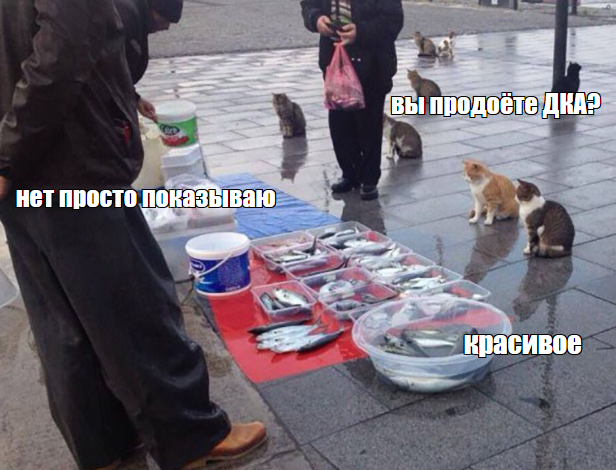
\includegraphics[]{img/DKA.png}
\end{center}

\newpage

\section{Определить, является ли язык регулярным}

\subsection{$L = \{(aab)^nb(aba)^m \: | \: n \geq 0, m \geq 0\}$}

Мы беспамятные уб... 

А, тут все ок. Тогда просто построим ДКА:

\digraph[scale=0.8]{g41}{
    size="6,6";
    rankdir="LR";
    node [shape=point]; 0;
    node [shape=circle]; 1 2 3 4 6 7;
    node [shape=doublecircle]; 5 8;
    0 -> 1;
    1 -> 2 [label="a"];
    2 -> 3 [label="a"];
    3 -> 4 [label="b"];
    4 -> 2 [label="a"];
    4 -> 5 [label="b"];
    5 -> 6 [label="a"]
    6 -> 7 [label="b"]
    7 -> 8 [label="a"];
    8 -> 6 [label="a"]
}

\subsection{$L = \{uaav \: | \: u \in \{a, b\}^{*}, v \in \{a, b\}^*,  |u|_b \geq |v|_a\}$}

\begin{enumerate}
    \item Рассмотрим отрицание языка $\Rightarrow \overline{L} = \{uaav \: | \: u \in \{a, b\}^{*}, v \in \{a, b\}^*,  |u|_b < |v|_a\}$ 
    \item Фиксируем $n \in N$.
    \item Берем $w = b^naaa^n$
    \item $|w| = 2(n + 1) > n$
    \item Рассмотрим разбиение:
    
    $x = b^{n - l}$
    
    $y = b^l$
    
    $|xy| = n; \: 0 < l < n \Rightarrow |y| \geq 1$
    
    $z = aaa^n$
    
    \item $\forall i \geq 0: xy^iz \in \overline{L}$ - не выполняется, так как уже при $i \geq 2 \Rightarrow |b^{n - l}b^{2l}| = n + l > n$.
    \item Делаем вывод, что язык нерегулярный, так как его отрицание не является регулярным.
\end{enumerate}

\subsection{$L = \{a^mw \: | \: w \in \{a, b\}^{*}, 1 \leq |w|_b \leq m\}$}

\begin{enumerate}
    \item Рассмотрим отрицание языка $\Rightarrow \overline{L}=\{a^mw | w \in \{a,b\}^*, |w|_b > m\}$
    \item Фиксируем $n \in N$.
    \item Берем $w = a^nb^n$
    \item $|w|= 2n \geq n$
    \item Рассмотрим разбиение:
    
    $x = a^{l}$
    
    $y = a^{k}$
    
    $|xy| = l + k \leq n; \: |y| \geq 1$
    
    $z = a^{n - l - k}b^n$
    
    \item $\forall i \geq 0: xy^iz \in \overline{L}$ - не выполняется, так как уже при $i \geq 2 \Rightarrow |a^{l}a^{ik}a^{n - l - k}b^n = a^{n + k(i-1)}b^n| \Rightarrow |b^n| = |w|_b = n < m = (n + k)$.
    \item Делаем вывод, что язык нерегулярный, так как его отрицание не является регулярным.
\end{enumerate}

\subsection{$L = \{a^kw^ma^n \: | \: k = n \lor m > 0\}$}

\begin{enumerate}
    \item Фиксируем $n \in N$.
    \item Берем $w = a^{n - 1}ba^n$
    \item $|w| = 2n \geq n$
    \item Рассмотрим разбиение:
    
    $x = a^{n - 1 - l}$
    
    $y = a^{j}b$
    
    $|xy| = l + j + 1 \leq n; \: |y| = j + 1 \geq 1$
    
    $z = a^{n}$
    
    \item $\forall i \geq 0: xy^iz \in L$ - не выполняется, так как при $i \geq 2 \Rightarrow |a^{n - 1 - l}(a^jb)^2a^n| = |a^{n - 1 - l + 2j}b^2a^n| \Rightarrow n - 1 - l + 2j = k \neq n$. При $i = 0 \Rightarrow m = 0$
    \item То есть $k \neq n$ и $m = 0$, делаем вывод, что язык нерегулярный.
\end{enumerate}

\subsection{$L = \{ucv \: | \: u \in \{a, b\}^{*}, v \in \{a, b\}^*, u \neq v^R\}$}

\begin{enumerate}
    \item Фиксируем $n \in N$.
    \item Берем $w = a^nca^{2n}$
    \item $|w| = 3n + 1 \geq n$
    \item Рассмотрим разбиение:
    
    $x = a^{n - l}$
    
    $y = a^{l}$
    
    $|xy| = n - l + l = n \leq n; \: |y| = l \geq 1$
    
    $z = ca^{2n}$
    
    \item $\forall i \geq 0: xy^iz \in L$ - не выполняется, так как при $i = 2$ и $l = n \Rightarrow a^{n - l}a^{2l} = a^{n + l} = a^{2n} \Rightarrow u = v^R$.
    \item Делаем вывод, что язык нерегулярный.
\end{enumerate}

\newpage

\begin{thebibliography}{9}
    \addcontentsline{toc}{section}{\refname}
    \bibitem{Graphviz} Документация Graphviz [Электронный ресурс]. URL: \url{https://graphviz.org/documentation/}
    
    \bibitem{NEERC-IFMO} Вики-конспекты ИТМО [Электронный ресурс]. URL: \url{https://neerc.ifmo.ru/wiki/}
\end{thebibliography}

\end{document}

\usepackage[english,russian]{babel}